\documentclass[10pt,a4paper]{article}
\usepackage[utf8]{inputenc}
\usepackage[T1]{fontenc}
\usepackage[spanish,es-tabla]{babel}
\usepackage{amsmath}
\usepackage{graphicx}
\usepackage{booktabs}
\usepackage[margin=2cm]{geometry}
\usepackage[hidelinks]{hyperref}

\title{Ajuste de la tabla de transformación de puntajes PAES\\ de Ciencias -- Física}
\author{Raúl Ignacio Chacana León}
\date{\today}

\begin{document}
\maketitle

\section{Descripción del proyecto}
En este proyecto trabaje con la tabla de transformación de puntajes de la prueba PAES de Ciencias -- Física (Forma 163), que entrega el DEMRE \cite{demre2026}. La tabla dice cuantos puntos PAES le corresponden a cada puntaje bruto $P$, que es el numero de respuestas correctas (de 0 a 75). La idea que hay detrás de todo esto, es guardar esos datos en un archivo, leerlos con Python y buscar funciones matemáticas que se parezcan a la tabla, para poder hacer un modelo matemático que simule una transformación de puntaje.

Probé tres funciones y las ajuste con \texttt{curve\_fit} de scipy \cite{virtanen2020}:
\begin{align}
f_1(P) &= a + bP + cP^2 + dP^3 \label{eq:p3}\\
f_2(P) &= a + bP + cP^2 + dP^3 + eP^4 + fP^5 \label{eq:p5}\\
f_3(P) &= a + b\,\ln\!\left(\frac{P + c}{d - P}\right) \label{eq:logit}
\end{align}
Las dos primeras son polinomios, que dentro de la matemática son los mas simples de probar y que se suelen ajustar fácil a muchas curvas. La tercera la elegí después de graficar los datos: la curva sube rápido al principio, casi se aplana en el medio y vuelve a subir rápido al final, y esa forma se parece a una función logarítmica de este tipo (como una sigmoide ``al revés'').

\section{Como lo hice y casos borde}
Para comparar los ajustes use el $\chi^2$ \cite{bevington2003}:
\begin{equation}
\chi^2 = \sum_{P} \left(\frac{y_P - f(P)}{\sigma}\right)^2 , \qquad \chi^2_{red} = \frac{\chi^2}{N - k}
\end{equation}
donde $N$ lo vamos a tomar como el numero de datos y $k$ el numero de parámetros. Como la tabla viene con números enteros, tome $\sigma = 0{,}5$ como error de cada dato (el redondeo). También calcule el $R^2$ para tener otra referencia.

El caso borde mas importante fue $P=75$. Entre $P=74$ y $P=75$ el puntaje pasa de 930 a 1000, un salto de 70 puntos que es muy grande y difícil de entender, mientras que el paso anterior fue de solo 22. Como ese punto no sigue la forma de la curva, decid\'i no usarlo en el ajuste y después ver que predecía cada función para ese valor. Otro detalle es que, la prueba tiene 80 preguntas pero solo 75 cuentan, por eso $P$ llega hasta 75. 

\section{Resultados}
La Tabla~\ref{tab:chi2} muestra la calidad de cada ajuste y la Figura~\ref{fig:ajustes} muestra los datos con las tres curvas. Como las curvas son casi iguales y se tapan entre ellas, agregue abajo un gráfico de residuos para ver mejor las diferencias, así poder comparar cada una de ellas y analizar en que difieren o en que se asemejan para llegar al mejor modelo matemático posible.

\begin{table}[ht]
\centering
\caption{Comparación de los ajustes ($N=75$ datos, de $P=0$ a $P=74$). La ultima columna es la predicción para $P=75$, donde el valor real es 1000.}
\label{tab:chi2}
\begin{tabular}{lccccc}
\toprule
Función & $k$ & $\chi^2$ & $\chi^2_{red}$ & $R^2$ & $f(75)$ \\
\midrule
$f_1$, polinomio grado 3 & 4 & 8454 & 119 & 0,9993 & 939 \\
$f_2$, polinomio grado 5 & 6 & 4568 & 66 & 0,9996 & 950 \\
$f_3$, logit             & 4 & 5087 & 72 & 0,9996 & 952 \\
\bottomrule
\end{tabular}
\end{table}

\begin{figure}[ht]
\centering
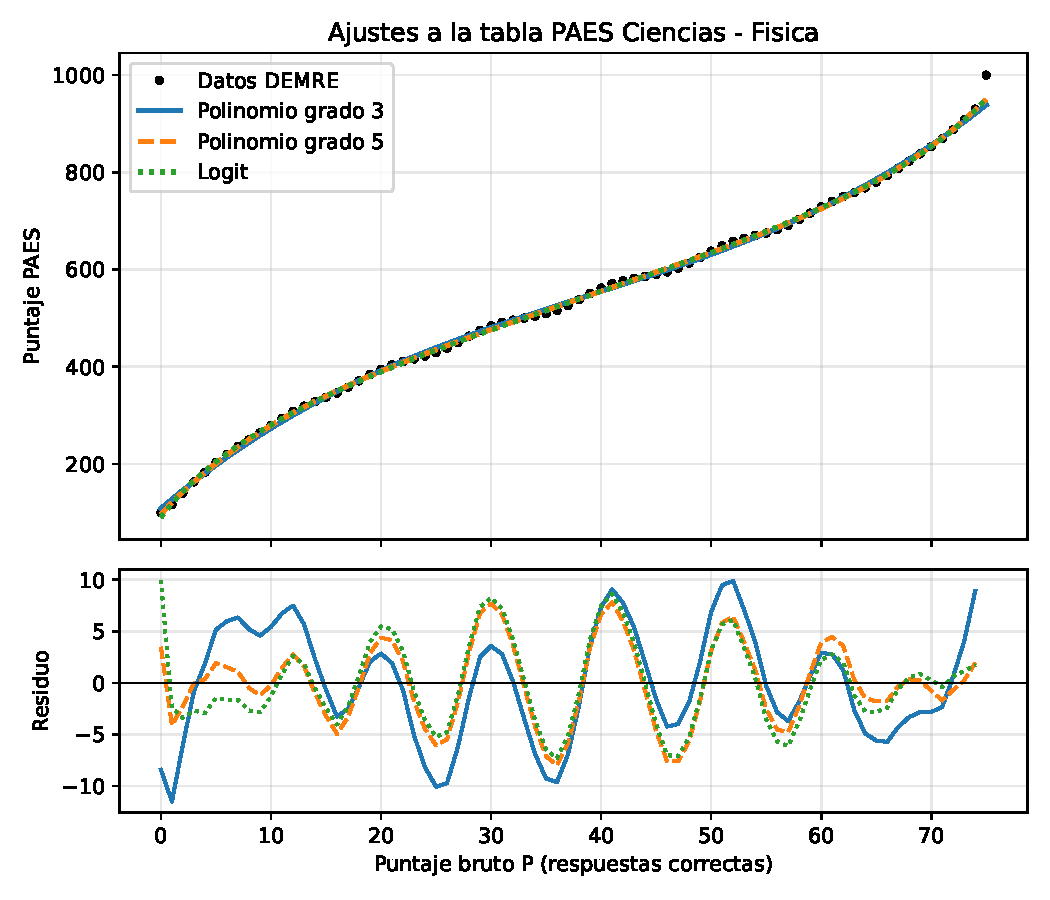
\includegraphics[width=0.5\textwidth]{figuras/ajustes_paes.pdf}
\caption{Arriba: datos del DEMRE (puntos negros) y las tres funciones ajustadas. Abajo: residuos (dato menos ajuste) de cada función.}
\label{fig:ajustes}
\end{figure}

Los parámetros que obtuvo el ajuste de $f_3$ fueron $a=540{,}5$, $b=172{,}9$, $c=6{,}09$ y $d=82{,}50$, es decir
\begin{equation}
\mathrm{PAES}(P) \approx 540{,}5 + 172{,}9\,\ln\!\left(\frac{P + 6{,}09}{82{,}50 - P}\right).
\end{equation}

\section{Discusión y reflexiones}
Dado que las tres funciones se ven muy parecidas a los datos en el gráfico y todas tienen $R^2$ sobre 0,999, uno se puede percatar que los $\chi^2_{red}$ son mucho mayores que 1, así que ninguna función es un ajuste perfecto (que dentro de todo, es lo que buscamos, algo que no sea perfecto, pero que se asemeje lo mas posible a la realidad), por eso, mi interpretación es que, la tabla del DEMRE no tiene como salir de una formula matemática, sino mas bien, lo podríamos ver como de un proceso estadístico, así que siempre va a tener pequeñas irregularidades que una curva suave no puede copiar. Por eso use el $\chi^2$ mas que nada para comparar las funciones entre si. El polinomio de grado 5 quedo con el menor $\chi^2$, pero el logit quedo casi igual usando solo 4 parámetros, así que me pareció una opción mejor y mas sensata para poder usarlo como transformación de puntaje.

Sobre $P=75$ me causo algo de confusión, dado que las tres funciones predicen entre 939 y 952, lejos de 1000. Esto me hizo pensar que el 1000 es un tope puesto a mano y no parte de la curva, así que fue buena idea sacarlo del ajuste para que me diera algo mas normal dentro de todo.

Y por ultimo, lo que mas me costo fue que \texttt{curve\_fit} necesita valores iniciales razonables: mi primer intento fue una sigmoide normal y los parámetros daban números sin sentido. Después de graficar los datos cambie de función y estime a ojo los parámetros de partida, así que de esto aprendí que graficar primero ayuda mucho a elegir el modelo. Así que a puro ensayo y error fueron saliendo las gráficas que se ajustaban a lo que uno buscaba.
\bibliographystyle{plain}
\bibliography{referencias}
\end{document}
